% =====================================================
% Placeholder: Table for Scaffold Reliability
% =====================================================
% \begin{table}[htb]
% \centering
% \scriptsize
% \begin{tabular}{llccc}
% \toprule
% Model & Retriever & Ours (No-CM) & Prior best & $\Delta$ \\
% \midrule
% OSS-120B          & AgentIR-4B & 79.4 & 67.0 & \textbf{+12.4} \\
% OSS-20B           & BM25       & 32.7 & 21.5 & \textbf{+11.2} \\
% Tongyi-DR   & AgentIR-4B & 80.7 & 68.1 & \textbf{+12.6} \\
% OR-30B    & Qwen3-8B   & 65.2 & 54.8 & \textbf{+10.4} \\
% \bottomrule
% \end{tabular}
% \caption{\hx{@Lei add one point and convert to figure}
% Our scaffold yields consistently higher \textit{No-CM} accuracy on BrowseComp-Plus than the highest publicly reported numbers for matched (model, retriever) pairs. ``Prior best'' is taken from~\citet{chen2025browsecompplus,team2025tongyideepresearch,li2026openresearcher,chen2026agentir}.
% All numbers are reported with accuracy (\%).
% }
% \vspace{-1em}
% \label{tab:scaffold-baseline}
% \end{table}


\begin{wrapfigure}{r}{0.4\linewidth}
\centering
    \vspace{-1.5em}
    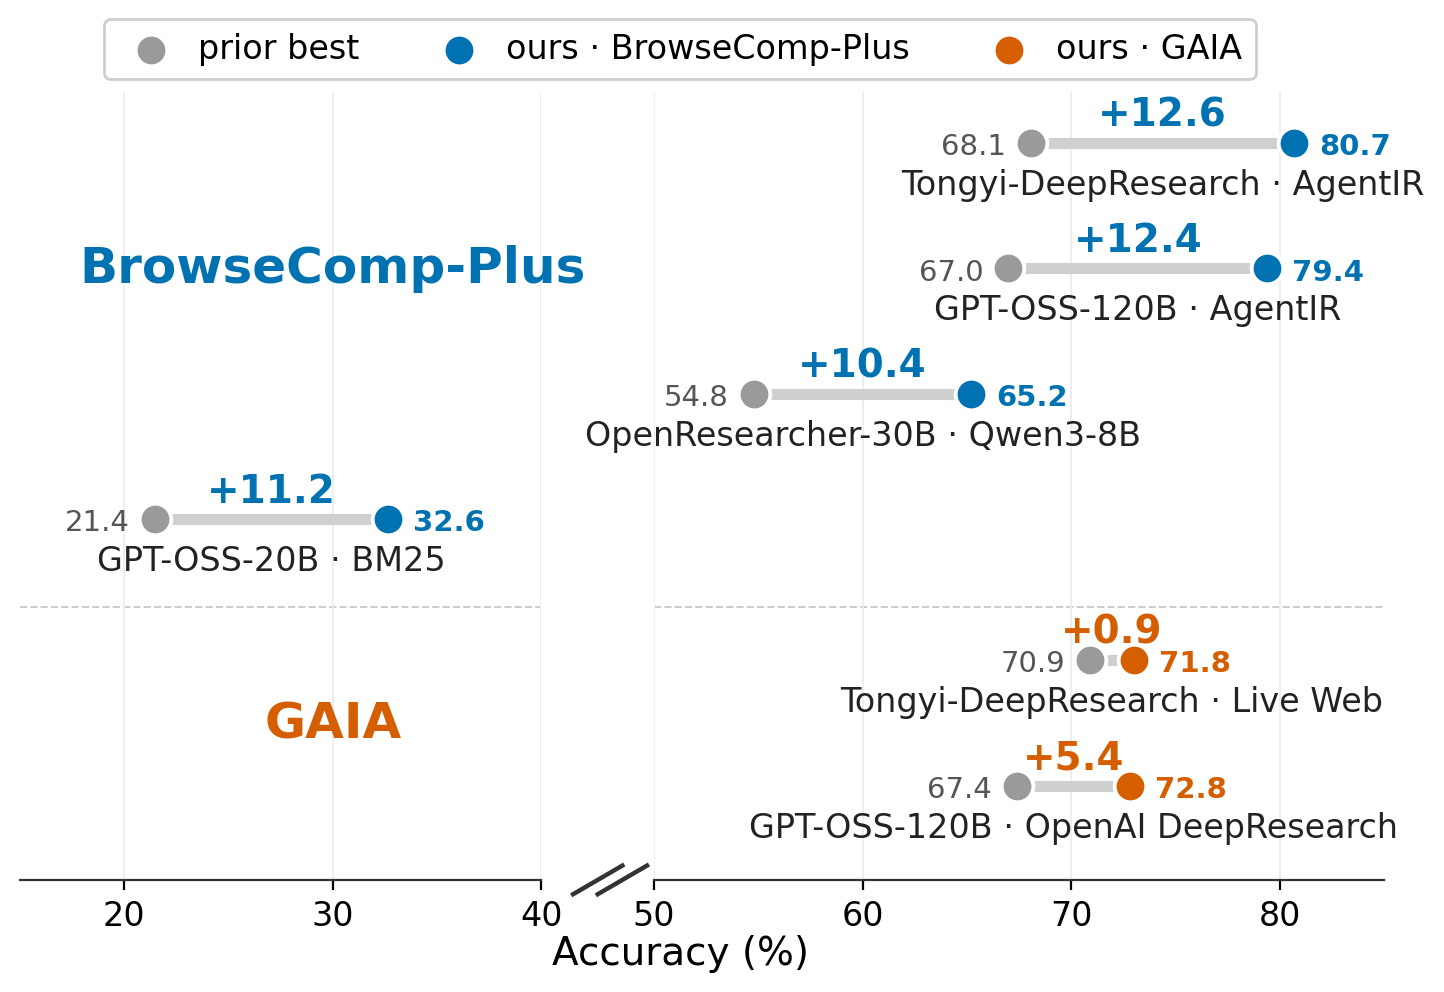
\includegraphics[width=\linewidth]{fig/reliability.png}
    \vspace{-2em}
    \caption{
Our scaffold consistently achieves higher \textit{No-CM} accuracy on BrowseComp-Plus and GAIA than the best publicly reported results for matched model--retriever pairs~\citep{chen2025browsecompplus,team2025tongyideepresearch,li2026openresearcher,chen2026agentir}.
% All results are reported as accuracy (\%).
}
\vspace{-3em}
\label{tab:scaffold-baseline}
\end{wrapfigure}